\chapter{January 12, 2021}

\section{Gravitational Waves}
\subsection{High energies (Raamis)}
Raamis showed his unblinding results for the optical counterpart. Raamis is working on the background trials for the large time windows he needs for discovery potential. Some are still finishing, but the curve has the proper behavior of looking flat for very short times and then beginning to asymptote towards a square root scaling. In plot, blue line is the maximum livetime that we have for the event selection.

\begin{figure}[h]
    \centering
    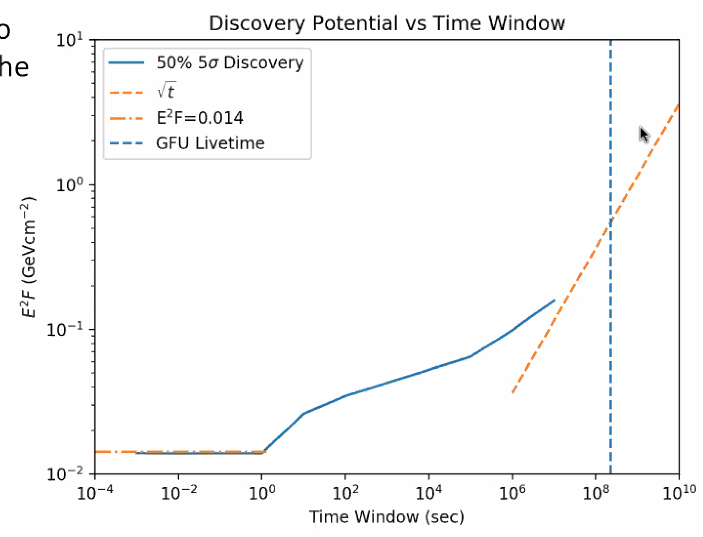
\includegraphics[width=0.6\textwidth]{images/raamis_plot_011221.png}
    \caption{Optical counterpart discovery potential vs. time. Vertical line is maximum allowed livetime by dataset. He is working on the few remaining time windows}
    \label{fig:my_label}
\end{figure}

\subsection{Lower energies (Aswathi)}
Aswathi fixed the sensitivity efficiency curve plot!!

The problem was with a seed, where the same seed was getting used each time, and when the computation time was split up there were not unique seeds in each job. Aswathi shows both sensitivity as well as discovery potential. 

\begin{figure}[h]
    \centering
    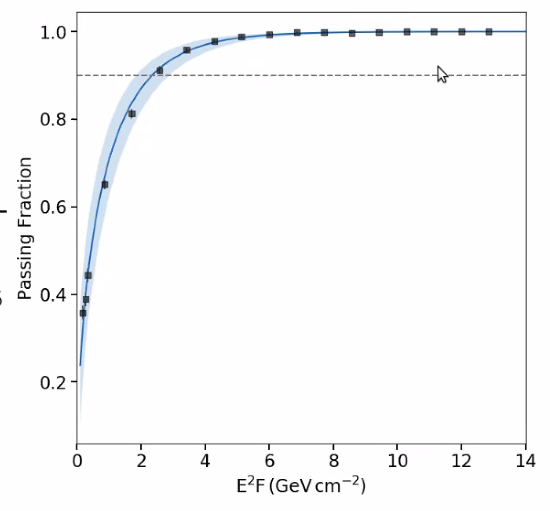
\includegraphics[width=0.6\textwidth]{images/aswathi_plot_011221.png}
    \caption{Aswathi's fixed sensitivity efficiency curve}
    \label{fig:my_label}
\end{figure}

\section{Novae, Fast Response, Millipede Maps, etc. (Alex)}

I prepared fast response paper responses for ApJ and am waiting to hear back from the internal review committee.

I also reached out to Chad who said he would review the alert followup analysis and send questions in the next week or so.

Millipede maps were discussed yesterday on the call. The working group seemed happy about the interpolation, and Erik seemed happy about reducing the resolution to save the computation time. I will work on implementing this in the next few weeks.

For novae, I showed that I am having some problems at longer timescales, and I think it is from the low stats in the background distribution at long time windows. 

\begin{figure}[h]
    \centering
    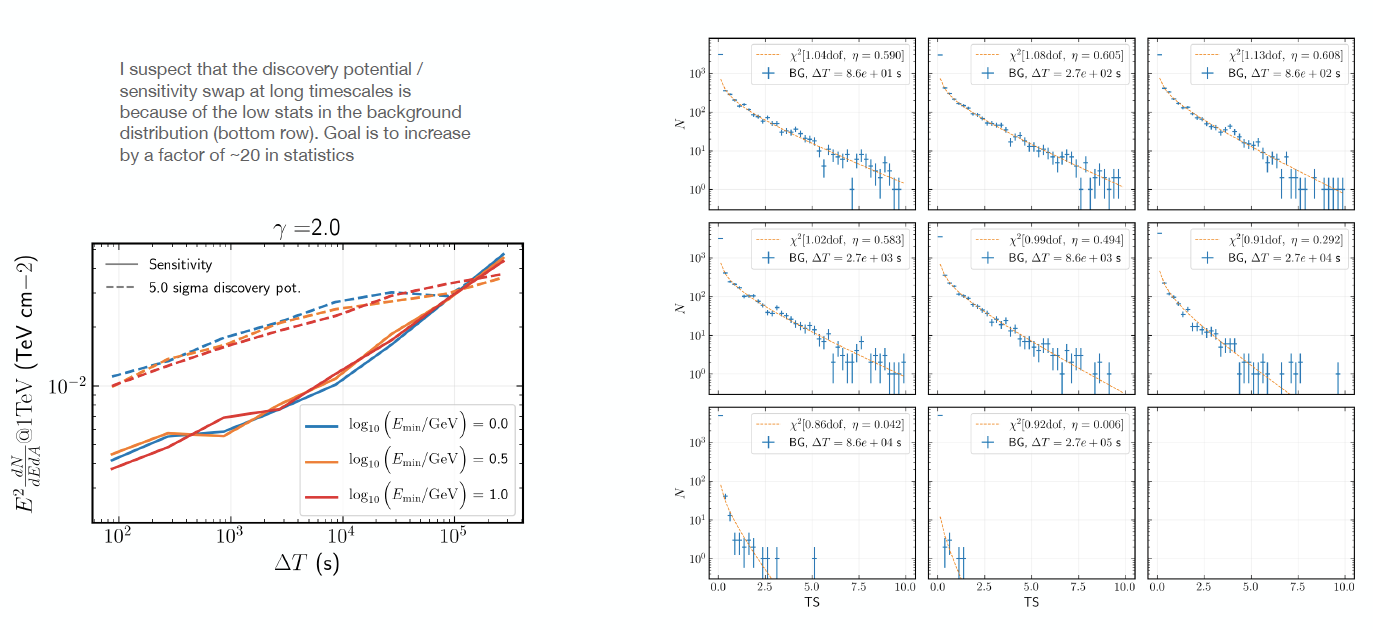
\includegraphics[width=0.6\textwidth]{images/alex_plot_011221.png}
    \caption{Novae plot showing that the background distributions (bottom right) at large time windows suffer from low stats because of the collapsing BG TS behavior.}
    \label{fig:my_label}
\end{figure}

\section{Radio Stacking (Abhishek)}
Abhishek looked more into the differential sensitivity. Some of the files were being moved around a few weeks ago when Abhishek made the last version of the plot and so the monte carlo weights were messed up. Now that things are fixed, he recalculated the differential sensitivity and around 100 TeV the sensitivity is at the level of a few 10s of percent of the diffuse flux

\begin{figure}[h]
    \centering
    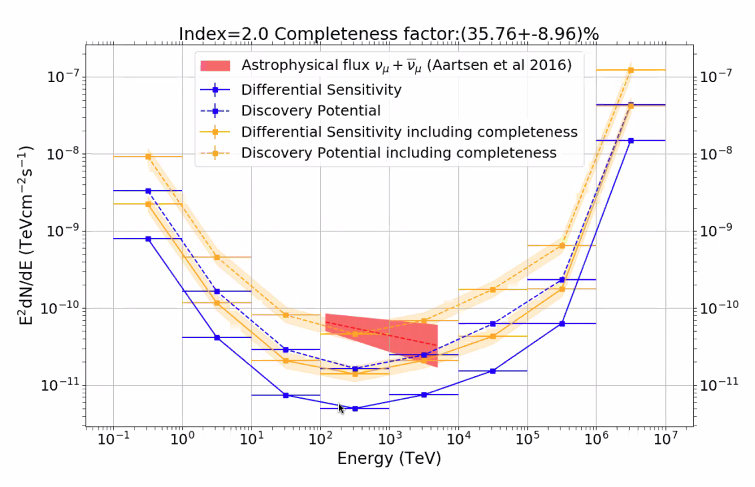
\includegraphics[width=0.6\textwidth]{images/abhishek_plot_011221.png}
    \caption{Abhishek's new differential sensitivity for radio stacking time-integrated}
    \label{fig:my_label}
\end{figure}

Abhishek is also working on calculating the central 90\% energy values for the single power law sensitivities.

Abhishek received questions from Federica and has responded to her and is waiting to hear back.

We also briefly discussed Abhishek's matrix of testing different hypotheses with the different injection schemes.

\section{ICRC Planning}
We discussed the ICRC planning and who will submit what topics. Topics to submit include:
\begin{enumerate}
    \item Aswathi: low energy GW
    \item Raamis: All high-energy analyses (tracks, realtime, optical, archival, maybe mention cascades). Could be broken up into a talk and a poster for current and upcoming
    \item Abhishek: Radio stacking
    \item Alex: I'm not sure yet?
\end{enumerate}